\section{Implementation}
\label{sec:framework:implementation}

\begin{figure}[ht]
\centering
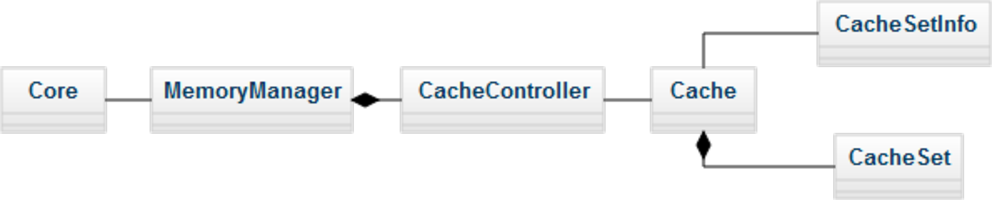
\includegraphics[scale=0.7]{figures/framework/functional_core_model}
\label{fig:framework:implementation:core_memory}
\caption{Partial core memory model in Sniper.}
\end{figure}

Figure~\ref{fig:framework:implementation:core_memory} shows an overview of the classes involved in the Sniper memory simulation.
The core class simulated the execution of instructions; this also includes simulating memory accesses to get and store instructions and data.
Each core as a memory manager instance which again, in our case, has four cache controllers.
A cache controller represents a single cache.
For shared caches, the cache controller instance in all but core 0 is a proxy, any calls to the proxy cache controllers is directed to the main controller at core 0.

When a core issues a memory request to the memory manager, the manager will issue the request to caches in order until it finds the data. 
If none of the caches have the requested data, the request is handled by the main memory simulation, which is not in the scope of this simplified overview.
Each cache controller knows its response latency and handles updating of the simulation time during each request.
In other words, the classes from Core down to CacheController handle a mix of functional and performance simulation.

Each cache controller has a cache instance, which is a purely functional cache model.
The cache class has methods for reading and writing to the cache, and each method returns whether the request was a hit or a miss.
This return value is then used by the CacheController to update the performance simulation.
Each cache is built from several CacheSet instances, each representing a single set, and possibly a single CacheSetInfo instance.
By modifying how the CacheSet operates, cache management algorithms can be implemented.
The CacheSetInfo instance is available to all cache sets and enables implementation of schemes that share data between cache sets.

In the original Sniper implementation, only the block tag requested is made available to the CacheSet. 
While this is enough to implement simple schemes, such as LRU and TADIP, we need more information to implement cache partitioning schemes such as UCP.
We have therefore modified Sniper by adding a data structure that is sent from the core when it initiates a memory request, all the way down to the cache set.
This data structure allows us to pass arbitrary data from the core to the cache set, allowing for more complex schemes.

\begin{figure}[ht]
\centering
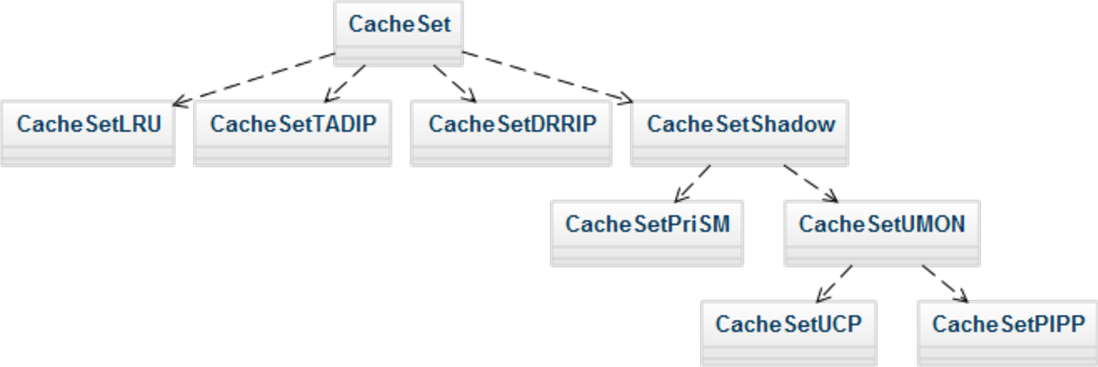
\includegraphics[scale=0.7]{figures/framework/algorithms}
\label{fig:framework:implementation:algorithms}
\caption{Implemented algorithms and their relations.}
\end{figure}

Of the schemes presented in Chapter~\ref{cpt:algorithms}, five have been implemented and tested in our simulation framework; LRU, TADIP-F, DRRIP-3, PriSM, UCP, and PIPP.

Figure~\ref{fig:framework:implementation:algorithms} shows how the five implemented algorithms relate to each other, and the base CacheSet class.
LRU, which is included in Sniper, and the two set dueling schemes TADIP and DRRIP, are all implemented as direct subclasses of the CacheSet class.
Based on the CacheSet class we have also implemented a cache with support for ATDs, also known as shadow tags.
By default, the ATDs do full sampling of the cache, but we made this configurable.
PriSM, which requires access statistics for each core, is implemented on top of the ATD implementation.
Also, we create a UMON implementation on top of the ATDs; this adds the utility calculating and block assigning functionality needed by both UCP and PIPP.
UCP and PIPP, are then implemented on top of the UMON base class.

Our implementation using inheritance reduces the number of code lines required when we implement multiple algorithms that share several properties.
By reducing the number of code lines required, we improve implementation time, and we reduce the chance of bug causing issues in our simulations.
Implementing additional algorithms in this framework requires only an understanding of the algorithm, as all of the simulator groundwork is already in place.
This makes the framework strongly suitable for future research.